\subsubsection{Card con los ingresos de la empresa}
Esta Card tiene distintos elementos que permiten ver la información de los ingresos en diferentes formatos.

Principalmente, en el encabezado de la Card se encuentran dos pestañas que, al darles clic, muestran la información de diferente manera. La pestaña por defecto es la que lleva por título ``Acumulado'', y en esta se muestra una gráfica de línea acumulada, es decir, una gráfica que muestra la suma acumulada de valores a lo largo del tiempo. Otro elemento importante en la manipulación de la gráfica es un botón que permite mostrar los valores en moneda o en cantidad, lo que también alterará como se ve la gráfica; el formato que está seleccionado por defecto es el de moneda.

Esta gráfica acumulada con formato de monto se ve de la siguiente manera (Ver Figura 29): 

    \begin{figure}[H]
        \begin{center}
            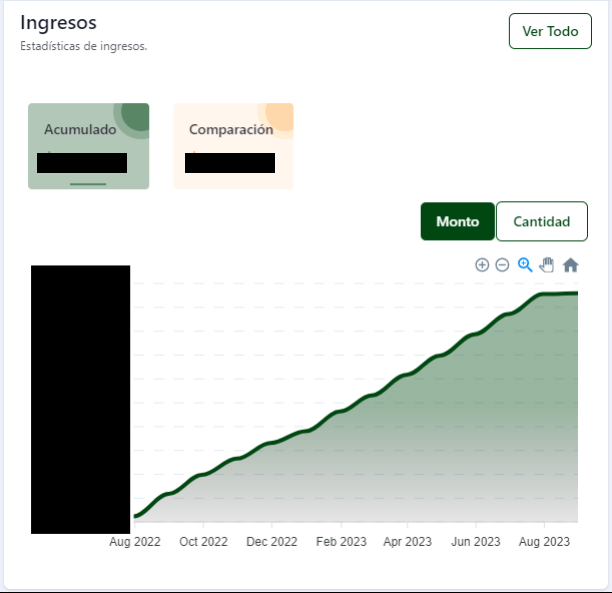
\includegraphics[scale=0.29]{img/actividades/dahsboard-admin/ingreso-acumulado-monto.png}
            \caption{Gráfica de línea acumulada con formato de moneda.}
            \label{fig:ingreso-acumulado-monto}
        \end{center}
    \end{figure}

Esta gráfica se verá alterada al cambiar el formato a cantidad, pues el conjunto de datos que se utiliza para generarla es diferente (Ver Figura 30).

    \begin{figure}[H]
        \begin{center}
            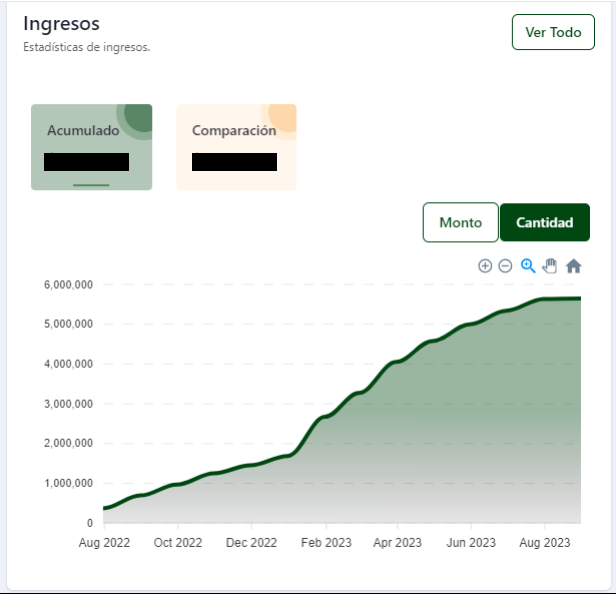
\includegraphics[scale=0.29]{img/actividades/dahsboard-admin/ingreso-acumulado-cantidad.png}
            \caption{Gráfica de línea acumulada con formato de cantidad.}
            \label{fig:ingreso-acumulado-cantidad}
        \end{center}
    \end{figure}

Para ver una comparación de ventas entre el año anterior y el actual, sólo es necesaro dar clic en la pestaña que tiene como título ``Comparación''. La gráfica que se presenta en esta pestaña también es de línea pero ya no es acumulativa, simplemente crece o se reduce de acuerdo a las ventas que se hayan realizado mes con mes, además, se muestran dos líneas para cada año. 

Al igual que en la pestaña anterior, es posible cambiar el formato en el que se presentan los datos, ya sea en moneda o en cantidad. La gráfica con formato de moneda se ve de la siguiente manera (Ver Figura 31): 

    \begin{figure}[H]
        \begin{center}
            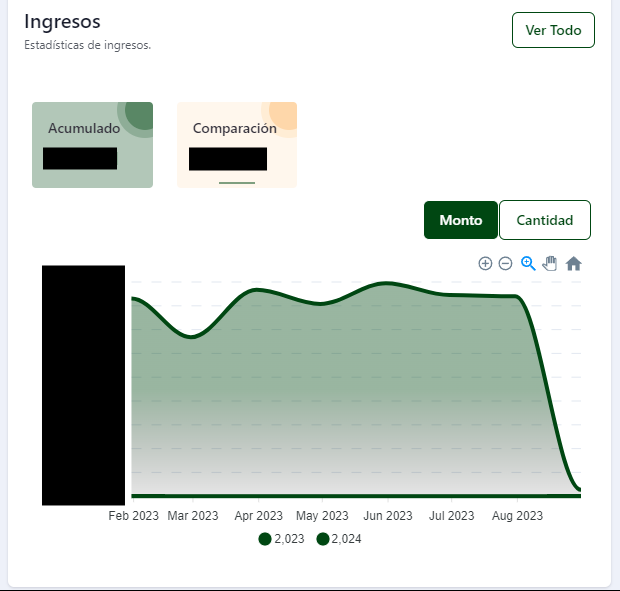
\includegraphics[scale=0.40]{img/actividades/dahsboard-admin/ingreso-comp-monto.png}
            \caption{Gráfica de línea comparativa con formato de moneda.}
            \label{fig:ingreso-comp-monto}
        \end{center}
    \end{figure}

Y la gráfica con formato de cantidad se ve así (Ver Figura 32): 

    \begin{figure}[H]
        \begin{center}
            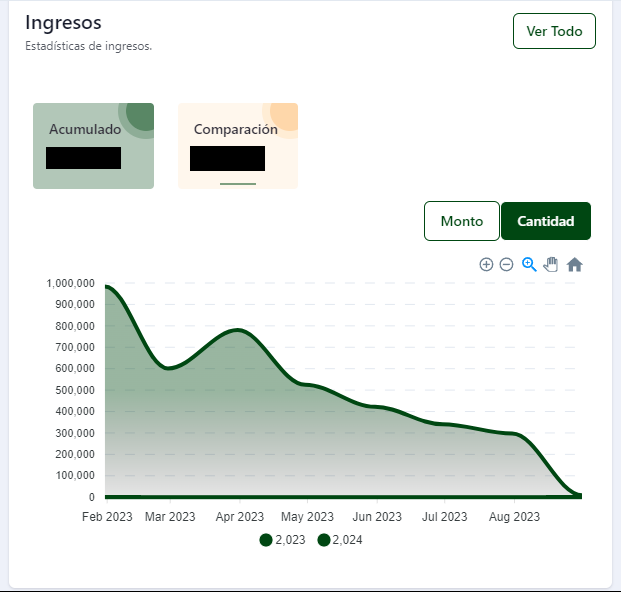
\includegraphics[scale=0.40]{img/actividades/dahsboard-admin/ingreso-comp-cantidad.png}
            \caption{Gráfica de línea comparativa con formato de cantidad.}
            \label{fig:ingreso-comp-cantidad}
        \end{center}
    \end{figure}